\chapter{ROOM Concepts}
\label{sec:room_concepts}

This chapter gives an overview over the ROOM language elements and their textual and graphical notation.
The formal ROOM grammar based on Xtext (EBNF) you can find in the \eTrice{} repository:
\url{http://git.eclipse.org/c/etrice/org.eclipse.etrice.git/plain/plugins/org.eclipse.etrice.core.room/src/org/eclipse/etrice/core/Room.xtext}

\section{Actors}

\subsection{Description}
 
The actor is the basic structural building block for building systems with ROOM. An actor can be refined 
hierarchically and thus can be of arbitrarily large scope. Ports define the interface of an actor.
An actor can also have a behavior usually defined by a finite state machine.

\subsection{Motivation}

\begin{itemize}
\item Actors enable the construction of hierarchical structures by composition and layering
\item Actors have their own logical thread of execution
\item Actors can be freely deployed
\item Actors define potentially re-usable blocks
\end{itemize}

\subsection{Notation}

\lstset{numbers=none, language=ROOM}

\begin{table}
\caption{Actor Class Notation}
\begin{tabular}{|l|l|l|}
\hline
 \textbf{Element} & \textbf{Graphical Notation} & \textbf{Textual Notation} \\ \hline
  ActorClass & 
  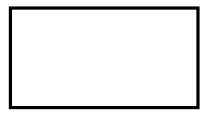
\includegraphics[scale=0.7]{images/040-ActorClassNotation.png} & 
  \begin{lstlisting}
ActorClass ActorClass2 {}
  \end{lstlisting}
\\ \hline
  ActorRef & 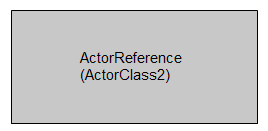
\includegraphics[scale=0.7]{images/040-ActorReferenceNotation.png} & 
  \begin{lstlisting}[language=ROOM]
ActorClass ActorClass1 {
  Structure {
    ActorRef ActorReference: ActorClass2
  }
}
  \end{lstlisting}
\\ \hline
\end{tabular}
\end{table}


\subsection{Details}

\subsubsection{Actor Classes, Actor References, Ports and Bindings}

An \room{ActorClass} defines the type (or blueprint) of an actor. Hierarchies are built by \room{ActorClass}es
that contain \room{ActorRef}erences which have another \room{ActorClass} as type. The interface of an 
\room{ActorClass} is always defined by \room{Port}s. The \room{ActorClass} can also contain
\room{Attribute}s, \room{Operation}s
and a finite \room{StateMachine}. 

External \room{Port}s define the external interface of an actor and are defined in the \room{Interface} 
section of the \room{ActorClass}.

Internal \room{Port}s define the internal interface of an actor and are defined in the \room{Structure} 
section of the \room{ActorClass}.

\room{Binding}s connect \room{Port}s inside an \room{ActorClass}.

Let us have a look at example \ref{tab:actor_class_example}:

\begin{table}
\caption{Actor Class Example}
\label{tab:actor_class_example}
\begin{tabular}{|l|l|l|}
\hline
 \textbf{Graphical Notation} & \textbf{Textual Notation} \\ \hline
 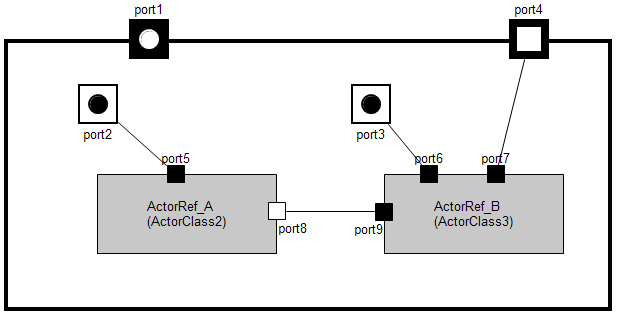
\includegraphics[scale=0.7]{images/040-ActorClass.png} & 
  \begin{lstlisting}
ActorClass ActorClass1 {
  Interface {
    Port port1: ProtocolClass1
    Port port4: ProtocolClass1
  }
  Structure {
    external Port port1
    conjugated Port port2: ProtocolClass1
    conjugated Port port3: ProtocolClass1
    ActorRef ActorRef_A: ActorClass2
    ActorRef ActorRef_B: ActorClass3
    Binding port2 and ActorRef_A.port5
    Binding port3 and ActorRef_B.port6
    Binding ActorRef_B.port7 and port4
    Binding ActorRef_A.port8 and ActorRef_B.port9
  }
}
  \end{lstlisting}
\\ \hline
 \end{tabular}
 \end{table}

\begin{itemize}
\item \textit{ActorClass1} contains two \room{ActorRef}erences (of ActorClass2 and ActorClass3)
\item \textit{port1} is an \textit{external end port}. Since it connects external actors with the behavior 
of the \room{ActorClass}, it is defined in the \room{Interface} section and the \room{Structure} section of 
the \room{ActorClass}.
\item \textit{port2} and \textit{port3} are \textit{internal end ports} and can only be connected to the 
ports of contained \room{ActorRef}erences. Internal end ports connect the behavior of an \room{ActorClass} with its 
contained \room{ActorRef}erences.
\item \textit{port4} is a relay port and connects external Actors to contained \room{ActorRef}erences. This port 
can not be accessed by the behavior of the \room{ActorClass}.
\item \textit{port5} through \textit{port9} are ports of contained actor references. \textit{port8} and 
\textit{port9} can communicate without interference with the containing actor class.
\item \room{Binding}s can connect ports of the actor class and its contained actor references. 
\end{itemize}

\subsubsection{Attributes}

\room{Attribute}s are part of the \room{Structure} of an actor class.
They can be of a \room{PrimitiveType} or a \room{DataClass}.

Example:

%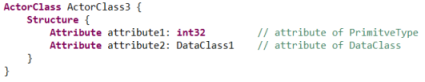
\includegraphics{images/040-ActorClassAttributes.png}
\begin{lstlisting}
ActorClass ActorClass3 {
  Structure {
    Attribute attribute1: int32       // attribute of primitive type
    Attribute attribute2: DataClass1  // attribute of DataClass type
  }
}
\end{lstlisting}

\subsubsection{Operations}

\room{Operation}s are part of the \room{Behavior} of an actor class.  Arguments and return values can be of a 
\room{PrimitiveType} or a \room{DataClass}. Data classes can be passed by value (implicit) or by reference (\room{ref}).

Example:

%\lstset{numbers=left, language=ROOM}

\begin{lstlisting}
ActorClass ActorClass4 {
  Behavior {
    // no arguments, no return value
    Operation operation1(): void {
      "UserCodeLine1"
    }
    // argument of primitive type, return value of primitive type
    Operation operation2(Param1: int32, Param2: float64): uint16 {
      "UserCodeLine1"
    }
    // arguments and return value by value
    Operation operation3(Param1: int32, Param2: DataClass1): DataClass1 {
      "UserCodeLine1"
    }
    // arguments and return value by reference except for primitive types
    Operation operation4(Param1: int32, Param2: DataClass1 ref): DataClass1 ref {
      "UserCodeLine1"
    }
  }
}
\end{lstlisting}

\section{Protocols}

\subsection{Description}

A \room{ProtocolClass} defines a set of incoming and outgoing \room{Message}s that can be exchanged between two ports.
The exact semantics of a message is defined by the execution model.

\subsection{Motivation}

\begin{itemize}
\item Protocol classes provide a reusable interface specification for ports
\item Protocol classes can optionally specify valid message exchange sequences
\end{itemize}

\subsection{Notation}

Protocol classes have only textual notation. 
The example defines a protocol class with 2 incoming and two outgoing messages. Messages can have data 
attached. The data can be of a primitive type (e.g. int32, float64, ...) or a data class.

%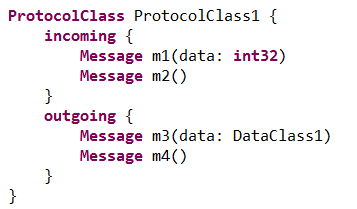
\includegraphics{images/040-ProtocolClassTextualNotation.png}
\begin{lstlisting}
ProtocolClass ProtocolClass1 {
  incoming {
    Message m1(data: int32}
    Message m2()
  }
  outgoing {
    Message m3(data: DataClass1}
    Message m4()
  }
}
\end{lstlisting}

\section{Ports}

\subsection{Description}

\room{Port}s are the only interfaces of actors. A port has always a protocol assigned. 
Service Access Points (SAP) and Service Provision Points (SPP) are specialized ports that are used to 
define layering.

\subsection{Motivation}

\begin{itemize}
\item Ports decouple interface definition (protocols) from interface usage
\item Ports decouple the logical interface from the transport 
\end{itemize}

\subsection{Notation}

\subsubsection{Class Ports}

These symbols can only appear on the border of an actor class symbol.

Ports that define an external interface of the actor class, are defined in the \room{Interface}. Ports 
that define an internal interface are defined in the \room{Structure} (e.g. internal ports).

\begin{itemize}
\item \textit{External end ports} are defined in the Interface and the Structure
\item \textit{Internal end ports} are only defined in the Structure
\item \textit{Relay ports} are only defined in the Interface
\item \textit{End ports} are always connected to the internal behavior of the ActorClass
\item \textit{Replicated ports} can be defined with a fixed replication factor, e.g.\\
\texttt{\room{Port} port18 [5]: ProtocolClass1}\\
or a variable replication factor, e.g.\\
\texttt{\room{Port} port18[*]: ProtocolClass1}
\end{itemize}

The table \ref{tab:class_port_notation} shows all kinds of class ports with textual and graphical notation.


\begin{longtable}{|m{2.5cm}|c|m{7cm}|}
\caption{Class Port Notation}
\label{tab:class_port_notation} \\
\hline
 \textbf{Element} & \textbf{Graphical Notation} & \textbf{Textual Notation}
\endhead
\hline
 \raggedright Class End Port & 
\includegraphics[scale=0.7]{images/040-ClassEndPort.png} & 
\begin{tabular}{l}
\textit{External Class End Port:} \\ 
%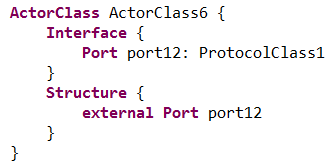
\includegraphics[scale=0.7]{images/040-ClassEndPortTextual.png}
\begin{lstlisting}
ActorClass ActorClass6 {
  Interface {
    Port port12: ProtocolClass1
  }
  Structure {
    external Port port12
  }
}
\end{lstlisting}
\\
\textit{Internal Class End Port:} \\ 
%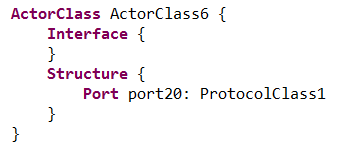
\includegraphics[scale=0.7]{images/040-ClassEndPortInternalTextual.png}
\begin{lstlisting}
ActorClass ActorClass6 {
  Interface {
  }
  Structure {
    Port port20
  }
}
\end{lstlisting}
\\
\end{tabular}
\\
\hline
 \raggedright Conjugated Class End Port & 

\includegraphics[scale=0.7]{images/040-ConjugatedClassEndPort.png} &
\begin{tabular}{l} 
\textit{External Conjugated Class End Port:} \\ 
\begin{lstlisting}
ActorClass ActorClass6 {
  Interface {
    conjugated Port port13: ProtocolClass1
  }
  Structure {
    external Port port13
  }
}
\end{lstlisting}
%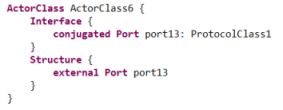
\includegraphics[scale=0.7]{images/040-ConjugatedClassEndPortTextual.png}
\\
\textit{Internal Conjugated Class End Port:} \\
\begin{lstlisting}
ActorClass ActorClass6 {
  Interface {
  }
  Structure {
    conjugated Port port21: ProtocolClass1
  }
}
\end{lstlisting}
%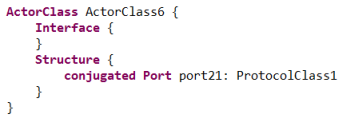
\includegraphics[scale=0.7]{images/040-ConjugatedClassEndPortInternalTextual.png}
\\ 
\end{tabular}
\tabularnewline
\hline
 \raggedright Class Relay Port &

\includegraphics[scale=0.7]{images/040-ClassRelayPort.png} & 
\begin{lstlisting}
ActorClass ActorClass6 {
  Interface {
    Port port10: ProtocolClass1
  }
  Structure {
  }
}
\end{lstlisting}
%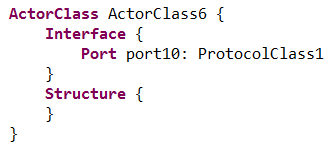
\includegraphics[scale=0.7]{images/040-ClassRelayPortTextual.png}
\tabularnewline
\hline
 \raggedright Conjugated Class Relay Port & 

\includegraphics[scale=0.7]{images/040-ConjugatedClassRelayPort.png} & 
\begin{lstlisting}
ActorClass ActorClass6 {
  Interface {
    conjugated Port port10: ProtocolClass1
  }
  Structure {
  }
}
\end{lstlisting}
%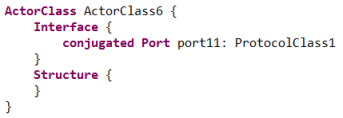
\includegraphics[scale=0.7]{images/040-ConjugatedClassRelayPortTextual.png}
\\
\hline
 \raggedright Replicated Class End Port & 

\includegraphics[scale=0.7]{images/040-ReplicatedClassEndPort.png} &
\begin{tabular}{b{5.5cm}} 
\textit{External Replicated Class End Port:} \\ 
\begin{lstlisting}
ActorClass ActorClass6 {
  Interface {
    Port port16[3]: ProtocolClass1
  }
  Structure {
    external Port port16
  }
}
\end{lstlisting}
%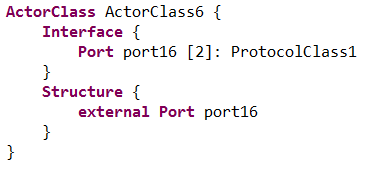
\includegraphics[scale=0.7]{images/040-ReplicatedClassEndPortTextual.png}
\\
\textit{Internal Replicated Class End Port:} \\
\begin{lstlisting}
ActorClass ActorClass6 {
  Interface {
  }
  Structure {
    Port port16[3]: ProtocolClass1
  }
}
\end{lstlisting}
%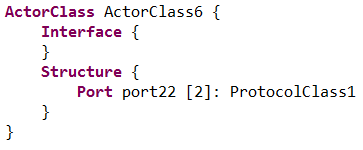
\includegraphics[scale=0.7]{images/040-ReplicatedClassEndPortInternalTextual.png}
\\ 
\end{tabular}
\tabularnewline
\hline
 \raggedright Conjugated Replicated Class End Port & 

\includegraphics[scale=0.7]{images/040-ConjugatedReplicatedClassEndPort.png} &
\begin{tabular}{b{5.5cm}} 
\textit{External Conjugated Replicated Class End Port:} \\ 
\begin{lstlisting}
ActorClass ActorClass6 {
  Interface {
    conjugated Port port17[3]: ProtocolClass1
  }
  Structure {
    external Port port17
  }
}
\end{lstlisting}
%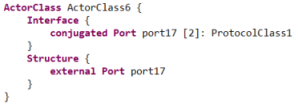
\includegraphics[scale=0.7]{images/040-ConjugatedReplicatedClassEndPortTextual.png}
\\
\textit{Internal Conjugated Replicated Class End Port:} \\ 
\begin{lstlisting}
ActorClass ActorClass6 {
  Interface {
  }
  Structure {
    conjugated Port port23[3]: ProtocolClass1
  }
}
\end{lstlisting}
%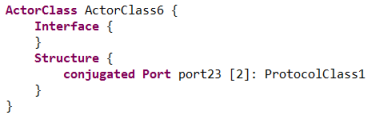
\includegraphics[scale=0.7]{images/040-ConjugatedReplicatedClassEndPortInternalTextual.png}
\\ 
\end{tabular}
\tabularnewline
\hline
 \raggedright Replicated Class Relay Port & 

\includegraphics[scale=0.7]{images/040-ReplicatedClassRelayPort.png} & 
\begin{lstlisting}
ActorClass ActorClass6 {
  Interface {
    Port port18[3]: ProtocolClass1
  }
  Structure {
  }
}
\end{lstlisting}
%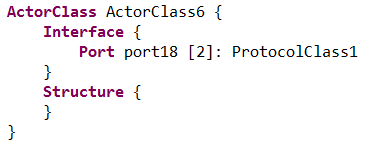
\includegraphics[scale=0.7]{images/040-ReplicatedClassRelayPortTextual.png}
\\ \hline
 \raggedright Conjugated Replicated Class Relay Port & 

\includegraphics[scale=0.7]{images/040-ConjugatedReplicatedClassRelayPort.png} & 
\begin{lstlisting}
ActorClass ActorClass6 {
  Interface {
    conjugated Port port19[3]: ProtocolClass1
  }
  Structure {
  }
}
\end{lstlisting}
%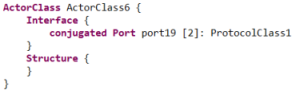
\includegraphics[scale=0.7]{images/040-ConjugatedReplicatedClassRelayPortTextual.png}
\tabularnewline
\hline
\end{longtable}


\subsubsection{Reference Ports}

These symbols can only appear on the border of an actor class. Since the type of port is defined 
in the actor class, no textual notation for the Reference Ports exists.

The table \ref{tab:reference_port_notation} shows all kinds of reference ports with textual and graphical notation.

\begin{table}
\caption{Reference Port Notation}
\label{tab:reference_port_notation}
\begin{tabular}{|c|c|c|}
\hline
 \textbf{Element} & \textbf{Graphical Notation} & \textbf{Textual Notation} \\ \hline
 Reference Port & 
\includegraphics{images/040-ReferencePort.png} & \textit{implicit} \\ \hline
 Conjugated Reference Port & 
\includegraphics{images/040-ConjugatedReferencePort.png} & \textit{implicit} 
\\ \hline
 Replicated Reference Port & 
\includegraphics{images/040-ReplicatedReferencePort.png} & \textit{implicit} 
\\ \hline
 Conjugated Replicated \\ Reference Port & 

\includegraphics{images/040-ConjugatedReplicatedReferencePort.png} & \textit{implicit} \\ \hline
\end{tabular}
\end{table}

\section{DataClass}

\subsection{Description}

The \room{DataClass} enables the modeling of hierarchical complex data types and operations on them.
The data class is the equivalent to a class in languages like Java or C++, but has less features. The content of a 
data class can always be sent via message between actors (defined as message data in a \room{ProtocolClass}).

\subsection{Notation}
  
Example: DataClass using PrimitiveTypes

\begin{lstlisting}
DataClass DataClass1 {
  Attribute attribute1: int32    // attribute of primitive type
  Attribute attribute2: float32  // attribute of another primitive type
  
  // no arguments, no return value
  Operation operation1(): void {
    "UserCodeLine1"
  }
  // argument of primitive type, no return value
  Operation operation2(Param1: int32): void {
    "UserCodeLine1"
  }
  // argument of primitive type, return value of primitive type
  Operation operation3(Param1: int32): float64 {
    "UserCodeLine1"
  }
}
\end{lstlisting}
%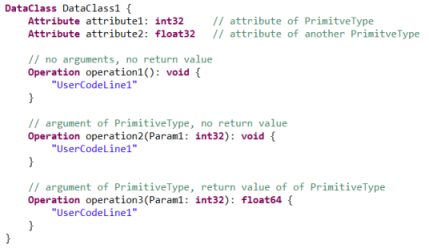
\includegraphics{images/040-DataClass1.png}

Example: DataClass using other DataClasses:

\begin{lstlisting}
DataClass DataClass2 {
  Attribute attribute1: int32      // attribute of primitive type
  Attribute attribute2: DataClass1 // attribute of DataClass
  
  // arguments and return value by value
  Operation operation1(Param1: int32, Param2: DataClass1): DataClass1 {
    "UserCodeLine1"
  }
  // arguments and return value by reference except for primitive types
  Operation operation2(Param1: int32, Param2: DataClass1 ref): DataClass1 ref {
    "UserCodeLine1"
  }
}
\end{lstlisting}
%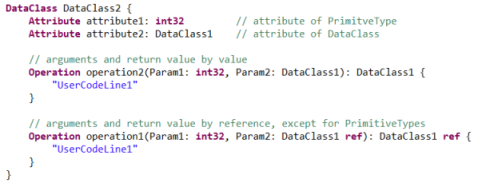
\includegraphics{images/040-DataClass2.png}

\section{Layering}

\subsection{Description}

In addition to the actor containment hierarchies, layering provides another method to hierarchically 
structure a software system. Layering and actor hierarchies with port to port connections can be mixed on 
every level of granularity.

\begin{enumerate}
\item an actor class can define a Service Provision Point (\room{SPP}) to publish a specific service, defined by a 
protocol class
\item an actor class can define a Service Access Point (\room{SAP}) if it needs a service, defined by a 
protocol class
\item for a given actor hierarchy, a \room{LayerConnection} defines which SAP will be satisfied by (connected to) 
which SPP
\end{enumerate}

\subsection{Notation}

For the graphical and textual notation refer to table \ref{tab:layering_notation}

\begin{table}
\caption{Layering Notation}
\label{tab:layering_notation}
\begin{tabular}{|m{3cm}|c|m{8cm}|}
\hline
\textbf{Description} & \textbf{Graphical Notation} & \textbf{Textual Notation} \\
\hline
\begin{flushleft}
	The layer connections in this model define which services are provided by the 
	\textit{ServiceLayer} (\textit{digitalIO} and \textit{timer})
\end{flushleft} &
% the raisebox centers the image vertically
\raisebox{-.5\height}{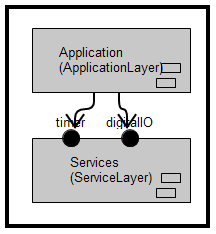
\includegraphics[scale=0.5]{images/040-LayeringModel.png}} & 
%\raisebox{-.5\height}{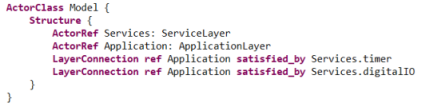
\includegraphics[scale=0.8]{images/040-LayeringModelTextual.png}}
\begin{lstlisting}
ActorClass Mode1 {
  Structure {
    ActorRef Services: ServiceLayer
    ActorRef Application: ApplicationLayer
    LayerConnection ref Application satisfied_by Services.timer
    LayerConnection ref Application satisfied_by Services.digitalIO
  }
}
\end{lstlisting}
\\
\hline
\begin{flushleft}
	The implementation of the services (SPPs) can be delegated to sub actors. In this case 
	the actor \textit{ServiceLayer} relays (delegates) the implementation services \textit{digitalIO} and 
	\textit{timer} to sub actors
\end{flushleft} & 
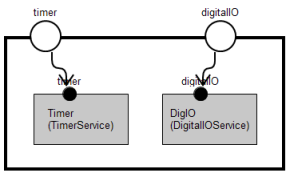
\includegraphics[scale=0.5]{images/040-LayeringServiceLayer.png} & 
%\raisebox{-.5\height}{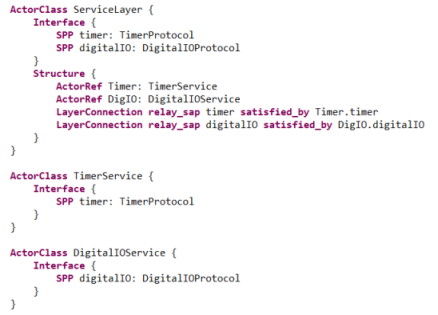
\includegraphics[scale=0.8]{images/040-LayeringServiceLayerTextual.png}}
\begin{lstlisting}
ActorClass ServiceLayer {
  Interface {
    SPP timer: TimerProtocol
    SPP digitalIO: DigitalIOProtocol
  }
  Structure {
    ActorRef Timer: TimerService
    ActorRef DigIO: DifitalIOService
    LayerConnection relay_sap timer satisfied_by Timer.timer
    LayerConnection relay_sap digitalIO satisfied_by DigIO.digitalIO
  }
}
\end{lstlisting}
\\
\hline
\begin{flushleft}
	Every Actor inside the \textit{ApplicationLayer} that contains an SAP with the same 
	protocol as \textit{timer} or \textit{digitalIO} will be connected to the specified SPP
\end{flushleft} & 
\raisebox{-.5\height}{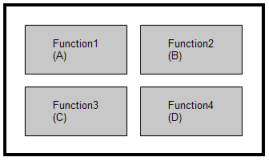
\includegraphics[scale=0.5]{images/040-LayeringApplicationLayer.png}} & 
%\raisebox{-.5\height}{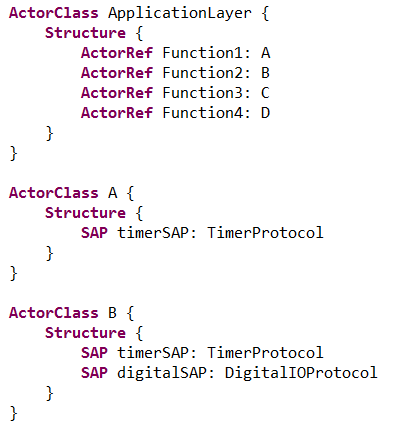
\includegraphics[scale=0.8]{images/040-LayeringApplicationLayerTextual.png}}
\begin{lstlisting}
ActorClass ApplicationLayer {
  Structure {
    ActorRef function1: A
    ActorRef function2: B
    ActorRef function3: C
    ActorRef function4: D
  }
}

ActorClass A {
  Structure {
    SAP timerSAP: TimerProtocol
  }
}

ActorClass B {
  Structure {
    SAP timerSAP: TimerProtocol
    SAP digitalSAP: DigitalIOProtocol
  }
}
\end{lstlisting}
\\
\hline
\end{tabular}
\end{table}

\section{Finite State Machines}

\subsection{Description}

Definition from \href{http://en.wikipedia.org/wiki/Finite-state\_machine}{Wikipedia}:

\begin{quote}
A finite-state machine (FSM) or finite-state automaton (plural: automata), or simply a state machine, is a 
mathematical model used to design computer programs and digital logic circuits. It is conceived as an 
abstract machine that can be in one of a finite number of states. The machine is in only one state at a 
time; the state it is in at any given time is called the current state. It can change from one state to 
another when initiated by a triggering event or condition, this is called a transition. A particular FSM 
is defined by a list of the possible states it can transition to from each state, and the triggering 
condition for each transition.

In ROOM each actor class can implement its behavior using a state machine. Events occurring at the end 
ports of an actor will be forwarded to and processed by the state machine. Events possibly trigger state 
transitions.
\end{quote}

\subsection{Motivation}

For event driven systems a finite state machine is ideal for processing the stream of events. Typically 
during processing new events are produced which are sent to peer actors.

We distinguish flat and hierarchical state machines.

\subsection{Notation}

We distinguish flat finite state machines (with just one level of hierarchy) and hierarchical ones.

\subsubsection{Flat Finite State Machine}

The simpler flat finite state machines are composed of the elements shown in table \ref{tab:flat_fsm_notation}.

\begin{table}
\caption{Flat finite state machine notation}
\label{tab:flat_fsm_notation}
\begin{tabular}{|m{3cm}|c|m{7cm}|}
\hline
\textbf{Description} & \textbf{Graphical Notation} & \textbf{Textual Notation} \\
\hline
State & 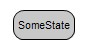
\includegraphics[scale=0.7]{images/040-State.jpg} &
\begin{lstlisting}
State SomeState
\end{lstlisting}
%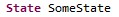
\includegraphics[scale=0.7]{images/040-StateTextual.jpg}
\\
\hline
 InitialPoint & 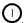
\includegraphics[scale=0.7]{images/040-InitialPoint.jpg} & \textit{implicit} \\
\hline
 TransitionPoint & 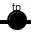
\includegraphics[scale=0.7]{images/040-TransitionPoint.jpg} & 
\begin{lstlisting}
TransitionPoint tp
\end{lstlisting}
%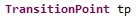
\includegraphics[scale=0.7]{images/040-TransitionPointTextual.jpg}
\\
\hline
 ChoicePoint & 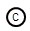
\includegraphics[scale=0.7]{images/040-ChoicePoint.jpg} & 
\begin{lstlisting}
ChoicePoint cp
\end{lstlisting}
%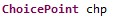
\includegraphics[scale=0.7]{images/040-ChoicePointTextual.jpg}
\\
\hline
 Initial Transition & \raisebox{-.5\height}{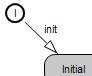
\includegraphics[scale=0.7]{images/040-InitialTransition.jpg}} & 
\begin{lstlisting}
Transition init: initial -> Initial { }
\end{lstlisting}
%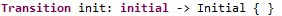
\includegraphics[scale=0.7]{images/040-InitialTransitionTextual.jpg}
\\
\hline
 Triggered Transition & 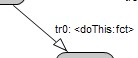
\includegraphics[scale=0.7]{images/040-TriggeredTransition.jpg} & 
\begin{lstlisting}
Transition tr0: initial -> DoingThis {
  triggers {
    <doThis: fct>
  }
}
\end{lstlisting}
%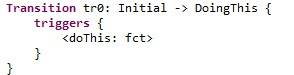
\includegraphics[scale=0.7]{images/040-TriggeredTransitionTextual.jpg}
\\
\hline
\end{tabular}
\end{table}


\subsubsection{Hierarchical Finite State Machine}

The hierarchical finite state machine adds the notion of a sub state machine nested in a state.
A few modeling elements listed in table \ref{tab:hier_fsm_notation} are added to the set listed above.

\begin{table}
\caption{Additional notation elements of hierarchical finite state machines}
\label{tab:hier_fsm_notation}
\begin{tabular}{|m{3cm}|c|m{7cm}|}
\hline
 \textbf{Description} & \textbf{Graphical Notation} & \textbf{Textual Notation} \\
\hline
 State with sub state machine &
\specialcell{Parent State \\ 
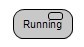
\includegraphics[scale=0.7]{images/040-StateWithSubFSM.jpg}} &
\begin{tabular}{l}
Sub state machine \\
\begin{lstlisting}
State Running {
  subgraph {
    Transition init: initial -> Process {}
    State Process
  }
}
\end{lstlisting}
\end{tabular}

%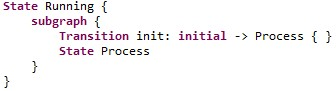
\includegraphics[scale=0.7]{images/040-StateWithSubFSMTextual.jpg}}
\\
\hline
 Entry Point &
 \specialcell{In sub state machine \\ 
\includegraphics[scale=0.7]{images/040-EntryPoint.jpg}} &
\begin{lstlisting}
EntryPoint reInit
\end{lstlisting}
%\includegraphics[scale=0.7]{images/040-EntryPointTextual.jpg}}
\\ \hline
 Exit Point & \includegraphics[scale=0.7]{images/040-ExitPoint.jpg} &
%\includegraphics[scale=0.7]{images/040-ExitPointTextual.jpg}
\begin{lstlisting}
ExitPoint tp0
\end{lstlisting}
\\ \hline
\end{tabular}
\end{table}

\subsection{Examples}

\begin{figure}
\includegraphics[scale=0.7]{images/040-FlatFSM.jpg}
\caption{Example of a flat finite state machine}
\end{figure}

\begin{figure}
\includegraphics[scale=0.7]{images/040-HierarchicalFSMTop.jpg}
\caption{Example of a hierarchical finite state machine -- top level}
\end{figure}

\begin{figure}
\includegraphics[scale=0.7]{images/040-HierarchicalFSMInitializing.jpg}
\caption{Hierarchical finite state machine -- sub state machine of \emph{Initializing}}
\end{figure}

\begin{figure}
\includegraphics[scale=0.7]{images/040-HierarchicalFSMRunning.jpg}
\caption{Hierarchical finite state machine -- sub state machine of \emph{Running}}
\end{figure}
